\section{Aufgabe 2}
\label{sec:Aufgabe2}
% \lstinputlisting[language=Python, firstline=15, lastline=21]{plots/plot.py}
\subsection{a)}
\begin{figure}[H]
  \centering
  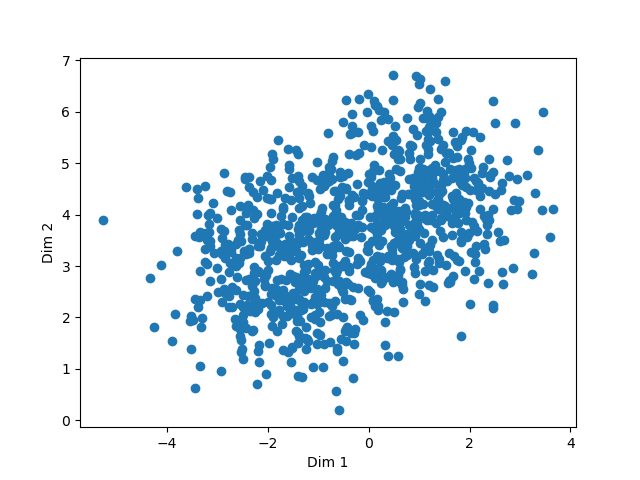
\includegraphics{plots/scatterplot_a.png}
  \caption{Scatterplot vor PCA}
  \label{fig:scatterplot}
\end{figure}
\subsection{b)}
Die PCA transformiert N Datenpunkte mit d Dimensionen auf k<d DImensionen.
Dafür werden die Größten Eigenwerte ausgewählt und aus den zugehörigen Eigenvektoren bilden die Transformationsmatrix in die neue Basis.
Die gesuchte neue Basis wird so festgelegt, dass die Varianz der Verteilung entlang der Basisvektoren maximiert wird.
Reihenfolge:
\begin{enumerate}
  \item Zentrierung der Daten $X$ um ihren Mittelwert
  \item Bestimmung der Kovarianzmatrix
  \item Diagonalisieren der Kovarianzmatrix
  \item Sortieren der Eigenwerte in absteigender Reihenfolge.
  \item Auswahl der k größten Eigenwerte und der zugehörigen Eigenvektoren.
  \item Bildung einer Matrix, in welcher die Eigenvektoren der k Ausgewählten Eigenwerte als Spalten stehen.
  \item Transfomation der Daten $X' = W X$ mithilfe der neuen Matrix $W$ um in ihrer Dimension reduzierte Daten zu erhalten.
\end{enumerate}

\subsection{c)}
Nichtsortierte Eigenwerte (mit linalg ausgerechnet):
\\
0.89875061  0.98813673  0.99958442 17.51933024
\\
Der vierte Eigenwert hebt sich deutlich von den anderen drei Eigenwerten ab.
\subsection{d)}

\begin{figure}
  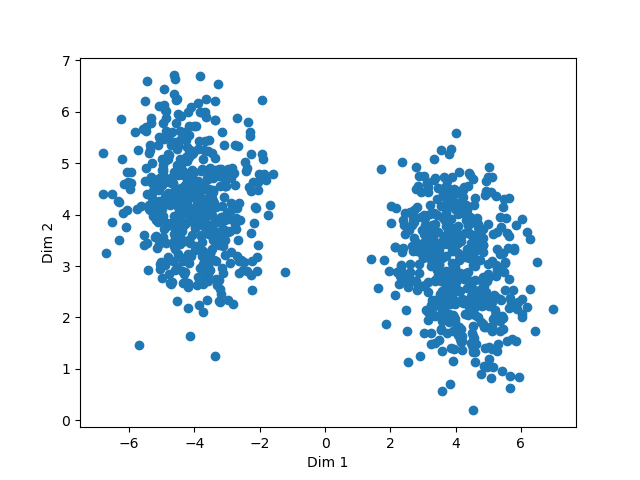
\includegraphics{plots/scatterplot_d.png}
  \caption{Scatterplot nach PCA}
  \label{fig:scatterplotnach}
\end{figure}

\begin{figure}
  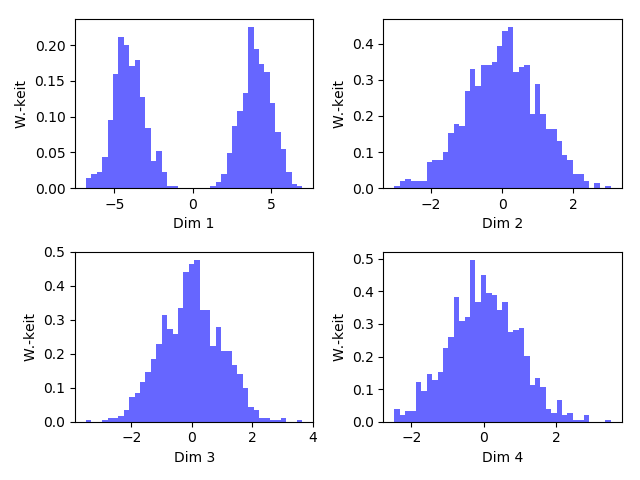
\includegraphics{plots/histogrammi.png}
  \caption{Histogramme der verschiedenen Dimensionen}
  \label{fig:hist}
\end{figure}
